\documentclass[runningheads,a4paper]{llncs}
\usepackage{amssymb}
\setcounter{tocdepth}{3}
\usepackage{graphicx}
\usepackage{algorithmic}
\usepackage{algorithm}

\usepackage{url}
%\urldef{\mailsa}\path|{andersonp,yongkiy,bernhardh,sowmya}@cse.unsw.edu.au|  
\newcommand{\keywords}[1]{\par\addvspace\baselineskip
\noindent\keywordname\enspace\ignorespaces#1}

\begin{document}

\mainmatter

\title{Robot Localisation Using Natural Landmarks}

%\titlerunning{Robot Localisation Using Natural Landmarks}

\author{Peter Anderson \and Yongki Yusmanthia \and \\
    Bernhard Hengst \and Arcot Sowmya}

%\authorrunning{Peter Anderson et al.}

\institute{School of Computer Science and Engineering,\\
University of New South Wales, UNSW Sydney 2052 Australia}

%\toctitle{Robot Localisation Using Natural Landmarks}
%\tocauthor{Peter Anderson}
\maketitle


\begin{abstract}
This paper introduces an optimised method for extracting natural landmarks to improve localisation during RoboCup soccer matches. The method uses modified 1D SURF features extracted from pixels on the robot's horizon. Consistent with the original SURF algorithm, the extracted features are robust to lighting changes, scale changes, and small changes in viewing angle or to the scene itself. Furthermore, we show that on a typical laptop 1D SURF runs more than one thousand times faster than SURF, achieving sub-millisecond performance. This makes the method suitable for visual navigation of resource constrained mobile robots. We demonstrate that by using just two stored images, it is possible to largely resolve the RoboCup SPL field end ambiguity. 
\end{abstract}


\section{Introduction}
In the RoboCup soccer Standard Platform League (SPL), the field set-up has changed over the years to progressively remove navigation beacons and other colour coded visual cues. In keeping with this trend, in the 2012 SPL competition the goal-posts at either end of the field are to be made the same colour for the first time. This implies that a robot forced to localise from an unknown starting position will not be able to resolve one end of the field from the other. In RoboCup matches this requirement can arise after a complicated fall, for example when robots become entangled, slip, and are rotated unwittingly. 

B-Human's 2011 Open Challenge demonstration addressed the field-end ambiguity challenge by using a team-wide ball model, enabling a kidnapped robot to recover by fusing their own ball observations with those of their team-mates \cite{thomas11code}. The authors acknowledged, however, that this approach could fail in situations where a robot is alone, unaware that it has been kidnapped, or if the team-wide ball model is incorrect. An own goal is the potentially disastrous result of one of these localisation failures. To avoid these problems and to allow a single robot to localise, a method for extracting unique natural landmarks from images of the unspecified environment beyond the field is required. In this context, a natural landmark is defined as a set of scale-invariant local features that can be used to find point correspondences, and ultimately a perspective transformation, between two images containing the same object.

SURF (Speeded Up Robust Features) \cite{bay2006SURF}, \cite{bay2008SURF} and SIFT (Scale-Invariant Feature Transform) \cite{lowe2004SIFT} are two existing methods for extracting invariant local features from images. However, these methods are relatively computationally expensive and difficult or impossible to implement in real time on a resource constrained robot. To overcome these resource limitations, this paper introduces an optimised feature detector consisting of a modified one dimensional SURF algorithm (1D SURF), applied to a single row of grey-scale pixels captured at the robot's horizon. The horizon image is chosen for analysis because, for a robot moving on a planar surface, the identified features cannot rotate or move vertically, and must always remain in the same order. The use of a 1D horizon image and other optimisations dramatically reduces the computational expense of the algorithm, while exploiting the planar nature of the robot's movement and still providing acceptable repeatability of the features. 

By using 1D SURF we show that a resource limited mobile robot is able to memorise and recognise natural landmarks seen at the horizon in typical indoor environments in real time.  Consistent with the original SURF algorithm, the extracted landmarks are robust to lighting changes, scale changes, small scene changes and small changes in viewing angle. We have used the Aldebaran Nao humanoid robot to evaluate the 1D SURF algorithm, but the method could be applied to other vision-based robot localisation problems where the robot moves on a planar surface and can estimate the position of the horizon in images. The remainder of this paper is organised as follows:  section \ref{sec:related} outlines related work, section \ref{sec:1DSURF} describes the 1D SURF algorithm and section \ref{sec:results} presents experimental results.


\section{Background}
 \label{sec:related}
Both SIFT \cite{lowe2004SIFT} and SURF \cite{bay2006SURF}, \cite{bay2008SURF} are feature representations that are designed to be stable under scale and viewpoint changes. Each method identifies potential features by searching for extrema at all possible scales of a grey-scale image. In SIFT, this step is implemented efficiently by using the difference of Gaussians function applied in scale-space to a series of smoothed and re-sampled images. Once features have been identified, they are accurately localised in both scale and location by interpolating from a 3D quadratic function fitted to local sample points. Next, feature points that are poorly located along an edge are eliminated and an orientation is assigned to each feature, so all future operations can be performed in a rotation invariant manner. SIFT calculates a 128-dimension descriptor vector for each identified feature based on the 8-bin histogram of the image gradient in 4x4 subregions around the feature point location. This, combined with the use of a Gaussian weighting function and normalisation of the descriptor vector, produces features that are invariant to scaling and rotation, as well as small viewpoint and illumination changes. 

SURF is related to SIFT, but instead of using a Difference of Gaussian filter, SURF uses simple box filters which can be evaluated very efficiently using integral images. Box filters are used to approximate Gaussian second order partial derivatives and find the determinant of the Hessian matrix, which is referred to as the blob response at a particular location and scale. Features are yielded at local maxima of this response, found by thresholding the response and applying non-maximal suppression in a 3x3x3 neighbourhood over the image and in scales. Like SIFT, SURF also involves feature localisation by interpolating from a fitted 3D quadratic function, and orientation assignment. The SURF feature descriptor uses integral images in conjunction with Haar wavelets to calculate a 64-dimension descriptor vector. This is calculated by summing both the signed and absolute values of both the horizontal and vertical Haar wavelet response over 25 sample points to generate a 4-dimension vector in each of 4x4 subregions around the feature point location. 

A comparison of SIFT and SURF using  a standard testing procedure based on a range of real-world images found SURF to be faster and more accurate than SIFT \cite{juan2009comparison}. For this reason we have chosen SURF as the basis of our 1D feature representation. Several other papers have adapted SIFT methods to operate on 1D data. The closest work to ours \cite{briggs2004scale}, \cite{briggs2006robot}, \cite{briggs2006matching}, use a 1D variation of SIFT to localise a mobile robot fitted with an omni-directional camera. This was achieved by identifying SIFT-like features in a 1D circular panoramic image, calculating feature descriptors based on colour and curvature information, and using a circular dynamic programming algorithm to match features between images. Compared to this work, we target a robot camera with a horizontal viewing angle of only 47.8 degrees, rather than 360 degrees, which dramatically reduces the amount of information available in a 1D horizon image. Furthermore, for reasons of computational efficiency we do not use colour information and use SURF rather than SIFT as the basis for our method. 

\section{1D SURF}
\label{sec:1DSURF}

In many respects the 1D SURF algorithm represents the equivalent of SURF, but using only one image dimension rather than two.  SURF searches for blob response extrema in a 3D scale-space consisting of horizontal location, vertical location and scale. In 1D SURF, the search is conducted in a 2D scale-space consisting of horizontal location and scale only. However, there are also some other significant modifications and simplifications which were made to the original algorithm, as outlined below. 

As indicated in Figure \ref{fig:horizon} Left, the input to the 1D SURF algorithm is a single row of grey-scale image pixels. The intensity values of these pixels are calculated by sub-sampling every 4 pixels along the robot's horizon, and taking the sum over a band of 30 vertical pixels at each sample point. The vertical sum minimises the sensitivity of extracted features to errors in the location of the horizon, and the sum is faster to compute than the mean. The resulting increase in pixel intensity values can be compensated in the response threshold. The position of the horizon in the image is determined by reading the robot's limb position sensors and calculating the forward kinematic chain from the foot to the camera, in accordance with the Denavit-Hartenberg parameters previously determined by the rUNSWift team \cite{HarDen55}.

\begin{figure} [h]
\begin{minipage}[b]{0.48\textwidth}
\centering
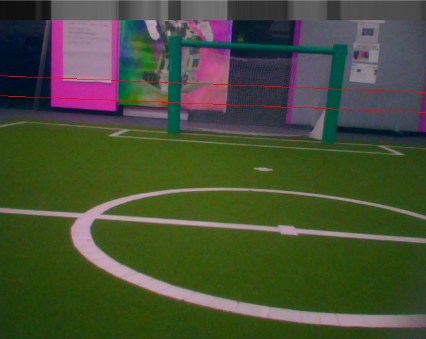
\includegraphics[width=1\textwidth]{figures/horizon.png}
\end{minipage}
\hspace{0.04\textwidth}
\begin{minipage}[b]{0.48\textwidth}
\centering
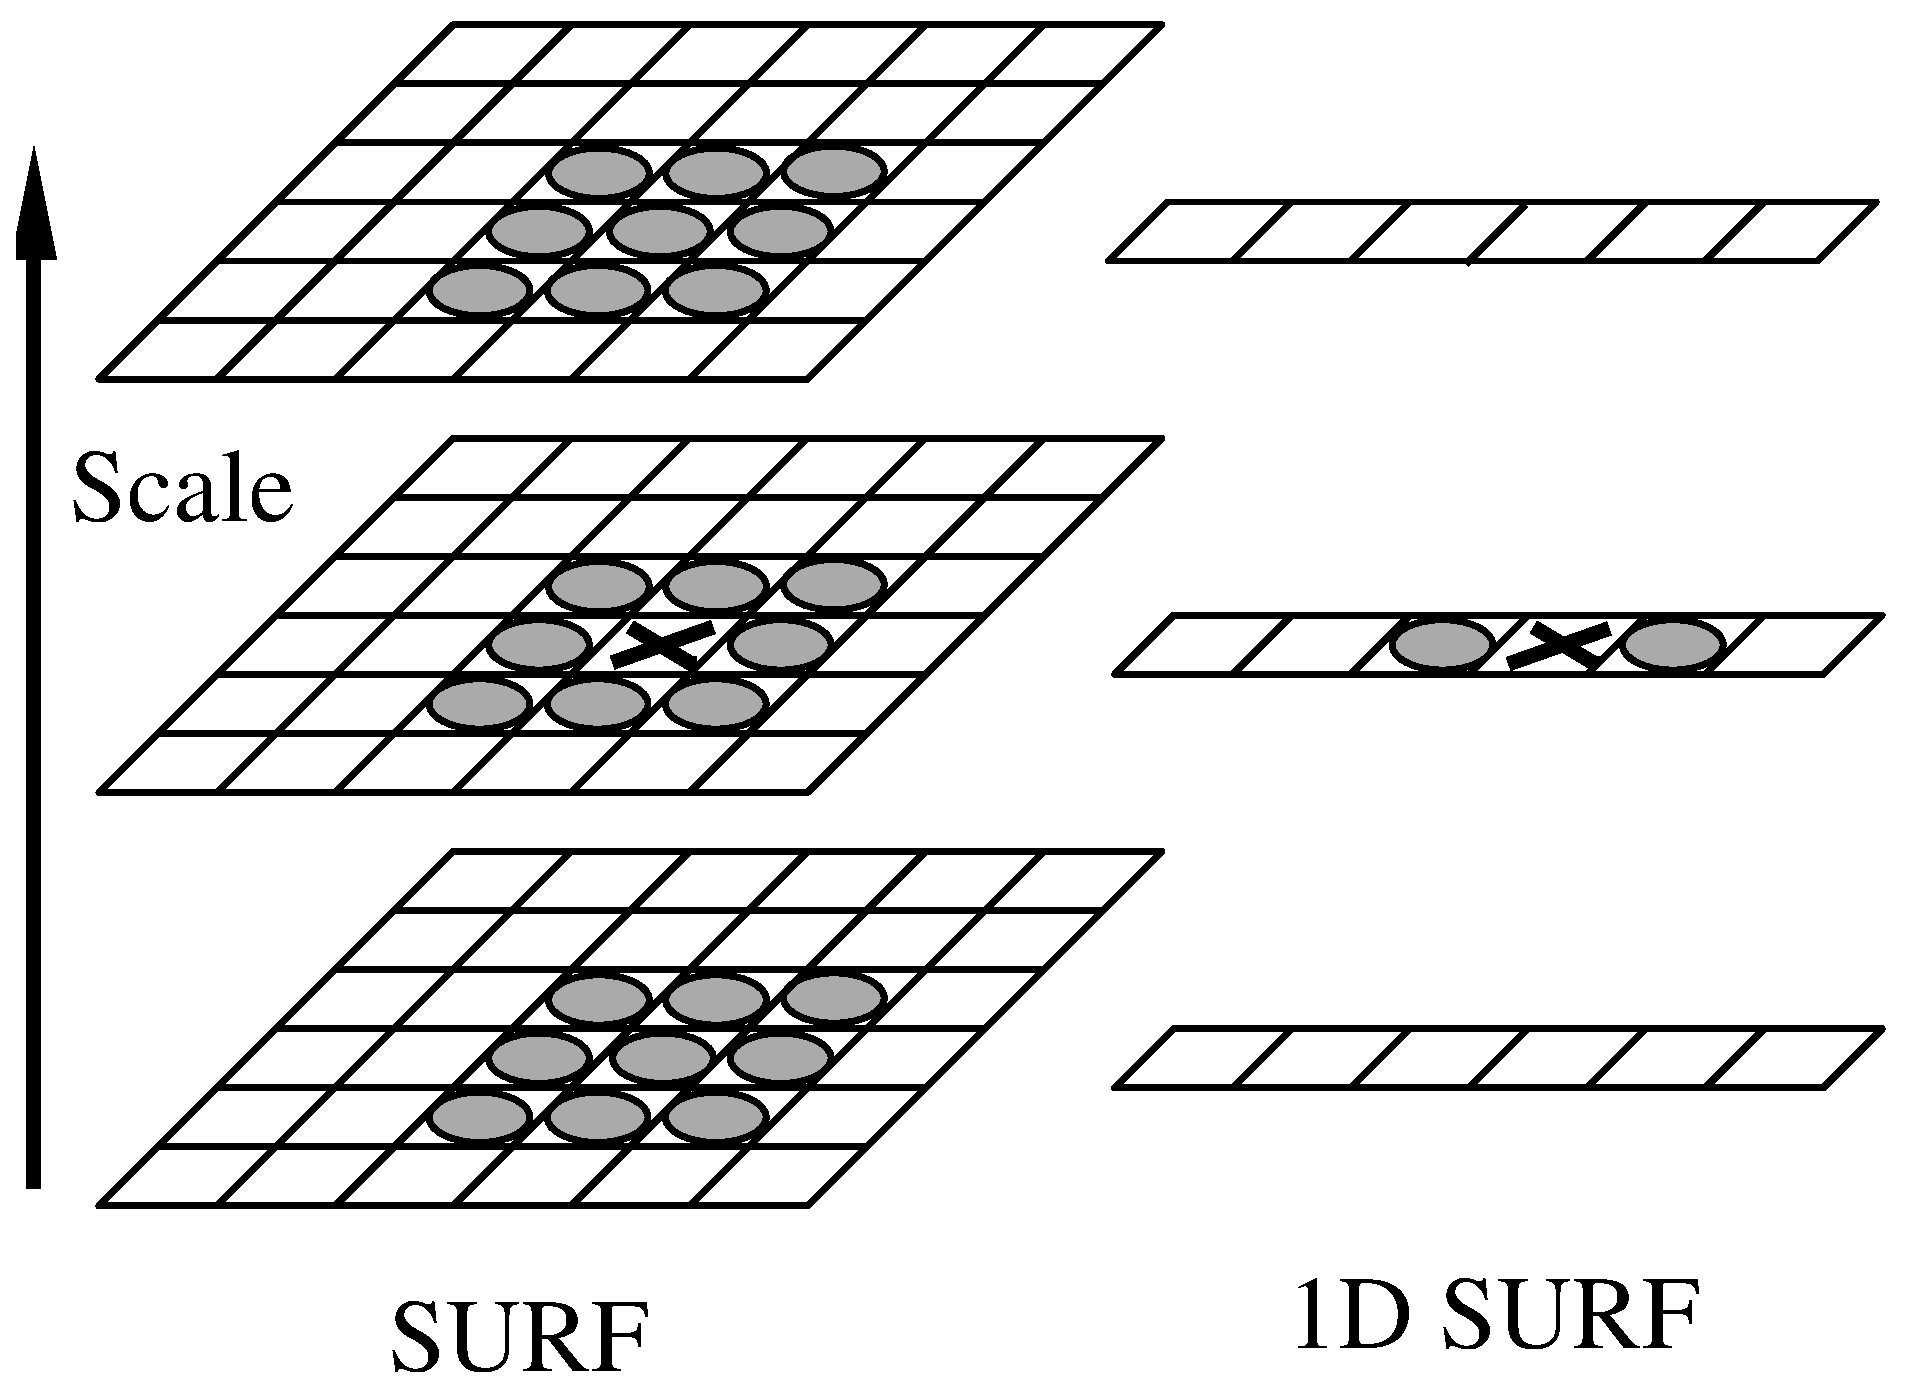
\includegraphics[width=1\textwidth]{figures/diagram}
\end{minipage}
\caption{Left: Image captured by the Nao robot showing superimposed 30 pixel horizon band in red, and the extracted grey-scale horizon pixels at the top of the image. Right: Identification of local maxima in scale-space. Pixel 'X' is selected as a maxima if it is greater than the marked pixels around it.} \label{fig:horizon}
\end{figure}

To identify local maxima of the blob response in scale-space, SURF thresholds the responses, then each pixel in 3D scale-space is compared to its 26 neighbours in a 3x3x3 neighbourhood to determine if it is a local maximum. In the case of 1D SURF, rather than searching for local maxima in a 3x3 scale-space neighbourhood, we apply a weaker test and only require that responses be extrema in the single space dimensional, as illustrated in Figure \ref{fig:horizon} Right. This relaxation ensures that sufficient feature points will be detected. It is an important aspect of the approach that a large number of relatively poor-quality features are generated, rather than relying on a small number of very distinctive features. A typical 1D horizon image containing 640 pixels might generate 50 - 70 features, depending on the parameter values chosen.  In our case we use a scale-space consisting of 4 octaves of 3 intervals each.

Since in 1D SURF all features are defined with reference to the horizon, the SURF orientation assignment step is no longer necessary and can be disregarded. SURF interpolates the location of features in both space and scale to sub-pixel accuracy by fitting a 3D quadratic curve to the local image function. In our application, we found that the additional accuracy provided by this step was not worth the computational burden, and it was also discarded. Finally, although the 1D SURF feature descriptor is calculated analogously to the SURF feature descriptor, due to the reduction in sample space and by using 3 subregions instead of 4, we produce a 6-dimension feature descriptor rather than a 64-dimension feature descriptor, allowing for much faster matching of descriptors across images. 


\subsection{Application to Natural Landmark Recognition}
A simple method is presented to memorise, and subsequently recognise, natural landmarks using 1D SURF features. Given a test image and a stored image, landmark recognition is performed by matching features in the test image to their nearest neighbours in the stored image, based on the Euclidean distance between feature descriptors. As before \cite{lowe2004SIFT}, feature matches are considered to be valid if the nearest-neighbour distance ratio is less than 0.7. Similarly \cite{briggs2006matching}, we then assign a recognition score to the test image calculated as the sum over all valid matched features of the inverse distance between feature descriptors. A high recognition score indicates that the test image contains the same natural landmark as the stored image with high likelihood. 

The above method, which we will refer to as nearest neighbour (NN) matching, does not preclude feature matches that are out of order, or otherwise inconsistent in terms of scale or horizontal displacement. Therefore a second matching method is presented, which first matches nearest neighbour features, and then uses RANSAC \cite{RANSAC} to discard feature matches that do not agree on a consistent landmark pose, before recalculating the recognition score. A consistent pose is defined as a set of matched features that conform to a straight line matching function as follows, where $x_{test,i}$ and $x_{stored,i}$ represent the horizontal pixel location of the $i$th matched feature in the test and stored images respectively, and $\beta_s$ and $\beta_d$ are scaling and displacement parameters: 

\begin{equation} \label{eq:1}
x_{test,i} = \beta_s x_{stored,i} + \beta_d
\end{equation}

\noindent
Given the robot's limited horizontal field of view, we find a straight line matching function is a reasonable approximation of the true feature matching function, which is curved in the presence of translation. Compared to NN matching, recognition scores calculated with this method will be lower, but have potentially greater discriminatory power. We will refer to this method as nearest neighbour matching with RANSAC (NN with RANSAC). The further advantage of this method is that it provides useful information about the robot's motion between the two images. The use of RANSAC to discard inconsistent matches generated by NN matching is shown in Figure \ref{fig:NN}.

\begin{figure} [h]
\begin{minipage}[b]{0.5\textwidth}
\centering
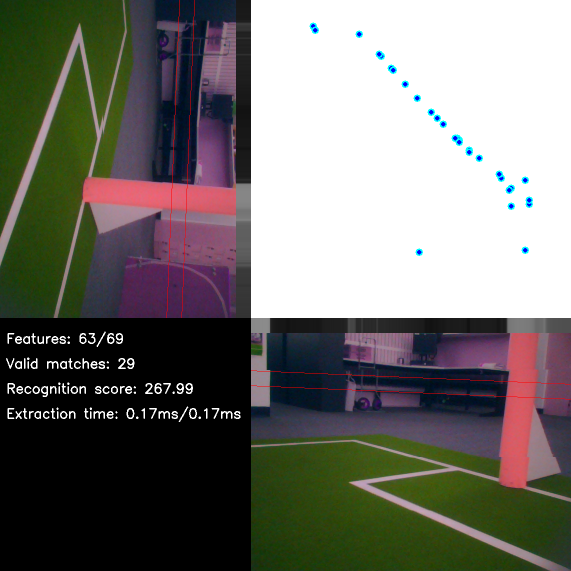
\includegraphics[width=1\textwidth]{figures/NN.png}
\end{minipage}
\begin{minipage}[b]{0.5\textwidth}
\centering
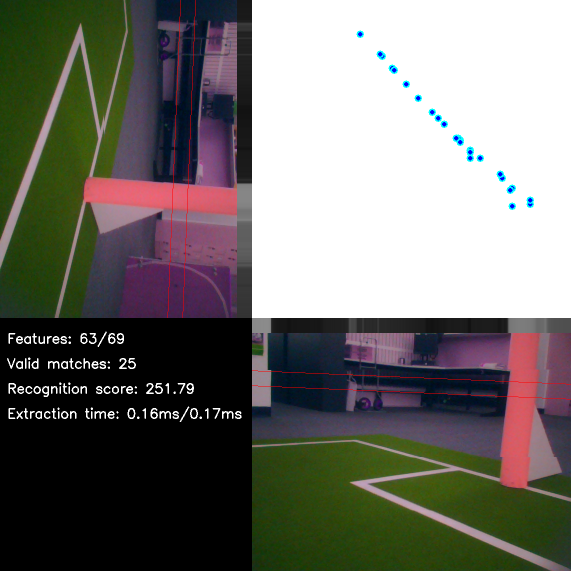
\includegraphics[width=1\textwidth]{figures/NNR.png}
\end{minipage}
\caption{Left: Matching features in two similar images based on nearest neighbour (NN) matching. Right: Matching features in the same two images after using RANSAC to discard matches that don't agree on a consistent pose (NN with RANSAC). As in Figure \ref{fig:horizon}, each image displays the horizon band in red and the extracted grey-scale horizon pixels at the top of the image. Matching features are plotted in the top-right panel against their horizon location in each image. The text panel illustrates the number of features detected in each image, the number of matches, the recognition score and the time taken to extract the features on a 2.4GHz laptop.}\label{fig:NN}
\end{figure}


\section{Experimental Results} 
\label{sec:results}

Two experiments were used to evaluate the performance of 1D SURF for robot localisation. In each experiment, the images used were captured using the Aldebaran Nao RoboCup edition v3.2, a humanoid robot equipped with a 500MHz AMD Geode LX800 processor. The Nao has two 640x480 pixel 30 fps digital cameras, each with a horizontal field of view of 47.8 degrees, which can be accessed one at a time. 

\subsection{Classification Experiment}
The first experiment was designed as a classification task, to assess whether the recognition score between two images could be used by the robot to determine whether both images contained the same landmark. Data for the experiment was captured by rotating the robot at a single location on the field, and capturing 88 images at approximately 4 degree increments. During this process the background around the field consisted of a typical office environment. From this image library we generated a test bank of 480 matched images and 2,065 unmatched images. Two images were considered to match if the angle between them was less than 20 degrees, implying at least 58\% of each image horizon overlapped with the other image. Example images from the test bank and the resulting recognition scores are shown in Figure \ref{fig:goodbad}.

\begin{figure} [h]
\begin{minipage}[b]{0.5\textwidth}
\centering
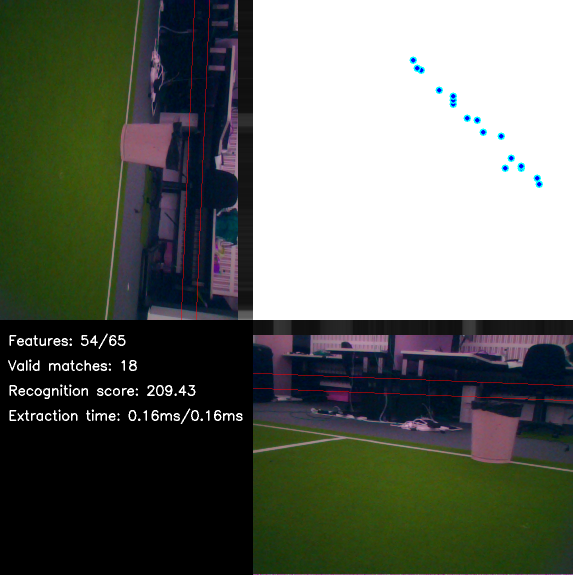
\includegraphics[width=1\textwidth]{figures/goodmatch.png}
\end{minipage}
\begin{minipage}[b]{0.5\textwidth}
\centering
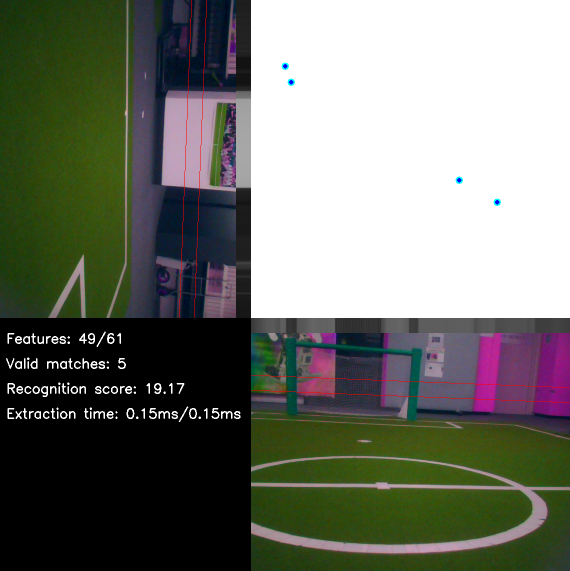
\includegraphics[width=1\textwidth]{figures/badmatch.png}
\end{minipage}
\caption{Left: Two images that almost completely overlap. Although the features on the horizon are not very distinctive, a high recognition score is generated using 1D SURF and NN with RANSAC feature matching. Right: Two images with no overlap, resulting in a low recognition score using the same method. As before, matching features are plotted in the top-right panel against their horizon location in each image, and the text panel contains key statistics.}\label{fig:goodbad}
\end{figure}

Although this experiment contains no changes in scale, illumination or viewing angle, it provides a useful baseline against which to tune parameters and assess the likely rate of false positive landmark recognitions.  Feature extraction and matching was performed off-board the robot using a 2.4GHz Core 2 Duo Processor laptop. This enabled the classification accuracy and speed of 1D SURF to be easily compared against SURF, for which we used the OpenSURF\footnote{http://www.chrisevansdev.com/computer-vision-opensurf.html} library implementation. 

The sensitivity and specificity  of SURF (using NN matching) and 1D SURF (using NN matching, and NN with RANSAC matching) with variation in the recognition score discrimination threshold is shown in Figure \ref{fig:ROC}. 1D SURF (using the horizon pixels only) is clearly less robust than SURF (processing the entire image). However, as illustrated in Table \ref{tab:speed}, 1D SURF uses only a fraction of the features, and runs more than one thousand times faster than SURF in this experiment. With the mean extraction time below 0.2ms, real-time feature extraction on the Nao during RoboCup soccer matches is a clear prospect. Also, using RANSAC to enforce a consist landmark pose results in a small improvement in classification accuracy.

\begin{figure} [h]
\centering
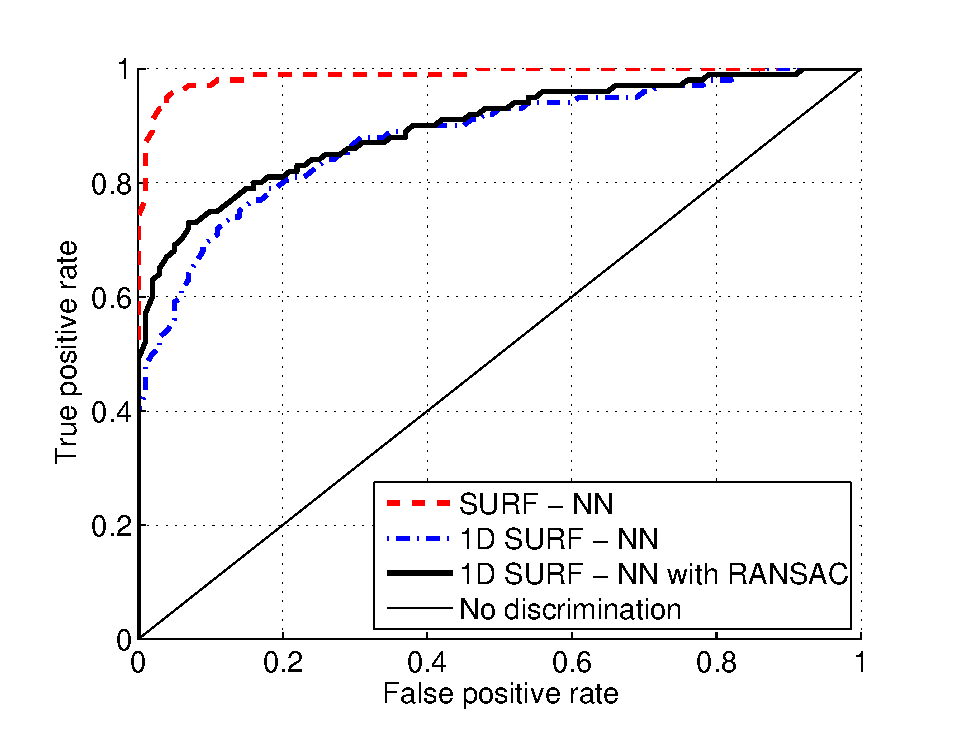
\includegraphics[width=0.6\textwidth]{figures/ROC}
\caption{ROC curve for classifying test images as matched or unmatched using the recognition score. Using NN with RANSAC matching on this data set, a threshold recognition score of 100 captured 70\% of true positives with a 5\% false positive rate. } \label{fig:ROC}
\end{figure}

\begin{table}
\caption{Running time of feature extraction and matching algorithms evaluated on a 2.4GHz Core 2 Duo laptop.}
\begin{tabular}{ p{1.8cm}p{4.2cm}p{1.2cm}p{1.5cm}p{1.45cm}p{1.6cm} }
\hline\noalign{\smallskip}
Feature extraction technique & Feature matching technique & Mean no. features & Mean extraction time (ms)  & Mean matching time (ms) & Area under ROC curve\\
\noalign{\smallskip}
\hline
\noalign{\smallskip}
SURF & Nearest neighbour (NN) & 429 & 222.3 & 19.1 & 98.8\% \\
1D SURF & Nearest neighbour (NN) & 59.2 & 0.158 & 0.069 & 88.0\% \\
1D SURF & NN with RANSAC & 59.2 & 0.158 & 0.076 & 89.6\% \\
\hline
\end{tabular}
\label{tab:speed}
\end{table}


\subsection{Field Experiment}
Having validated the performance of 1D SURF on highly similar images, the second experiment was designed to assess the performance of 1D SURF under changes in scale, viewing angle, illumination and with small scene changes. It was performed on-board the Nao robot to provide a clearer assessment of the processing speed of the method with constrained hardware. In this experiment, we used NN with RANSAC matching and evaluated 1D SURF the way it might be used in a SPL match; to distinguish one end of the field from the other. To do this, we positioned the Nao in the centre of the field, captured one image of each goal area, and stored the extracted feature vectors. Next, we moved the Nao through a 1m grid of positions covering a 4m x 4m area of the field (25 positions in total), and recorded the recognition scores at each point when manually positioned to face approximately towards each goal. By moving the Nao around the field, large changes in scale and viewing angle were generated. At each point we hoped to observe a large recognition score for the stored goal the robot was actually facing, and a low recognition score for the other goal, indicating that this technique could be used to reliably distinguish field ends during a match. During this entire experiment both goals were coloured yellow, and background objects were approximately 2m behind the goals themselves.

The recognition scores recorded during this exercise are overlaid on a field map in Figure \ref{fig:heatmap}. Using a recognition threshold of 100 (as determined during the classification experiment), each field end is correctly recognised from the single stored image in more than half of the 4m x 4m test area. A very strong recognition response (greater than 200) is observed in a radius of approximately 1m around the location of the original stored image. Finally, there were zero false positives recorded when facing the opposite end of the field. The recognition response to the opposite end of the field is almost always less than 50. Overall, these results indicate that even with just two stored images, a kidnapped robot could resolve one end of the field from the other from most mid-field positions. To provide a clearer indication of the field environment used during the experiment, Figure \ref{fig:examples} depicts the stored goal images and examples of views from different areas of the field. 

\begin{figure} [h]
\begin{minipage}[b]{0.5\textwidth}
\centering
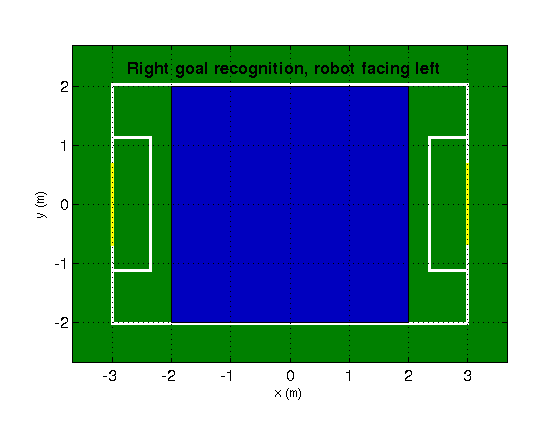
\includegraphics[width=1\textwidth]{figures/RL}
\end{minipage}
\begin{minipage}[b]{0.5\textwidth}
\centering
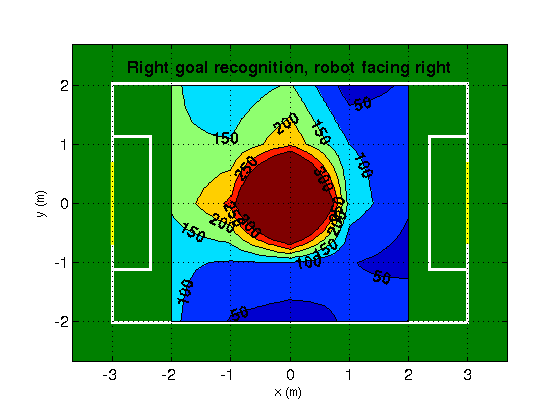
\includegraphics[width=1\textwidth]{figures/RR}
\end{minipage}
\begin{minipage}[b]{0.5\textwidth}
\centering
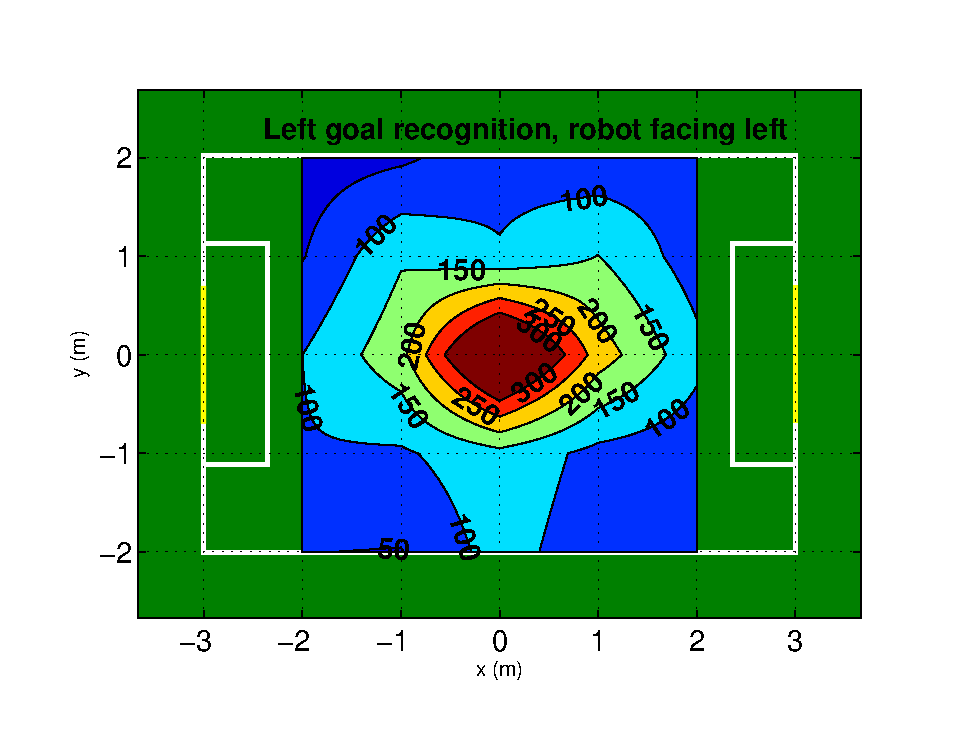
\includegraphics[width=1\textwidth]{figures/LL}
\end{minipage}
\begin{minipage}[b]{0.5\textwidth}
\centering
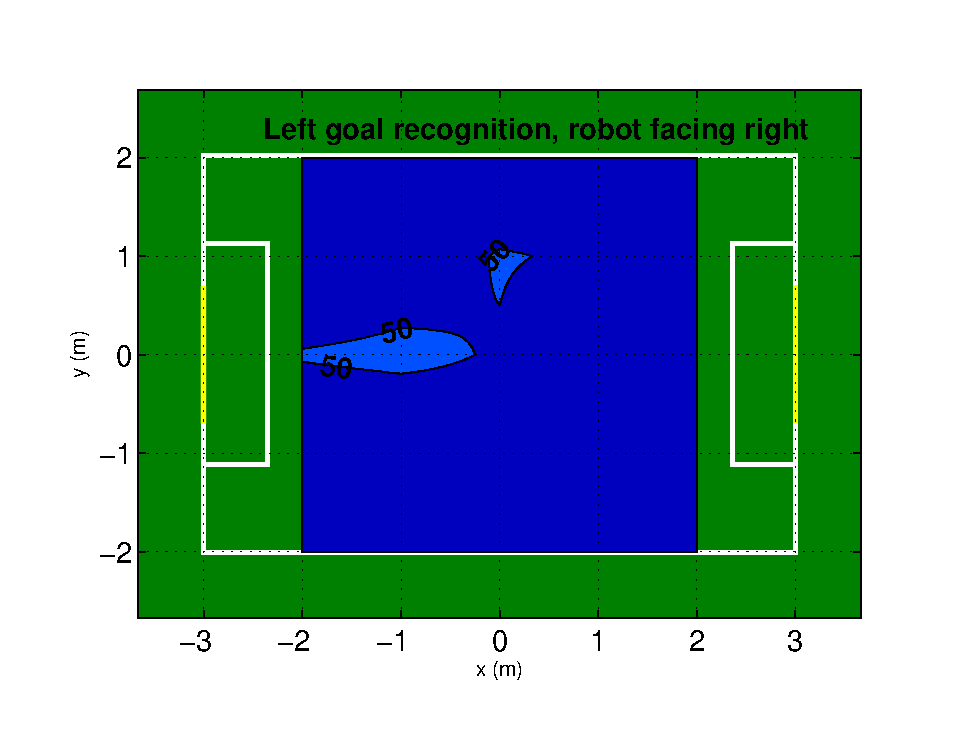
\includegraphics[width=1\textwidth]{figures/LR}
\end{minipage}
\caption{Recognition scores of a single goal image from different areas of the field. Clockwise from top left: Recognition of right-hand goal when facing left, recognition of right-hand goal when facing right, recognition of left-hand goal when facing right, recognition of left-hand goal when facing left.} \label{fig:heatmap}
\end{figure}

In many robot navigation applications, including RoboCup SPL, robots are subject to varied lighting conditions and the natural landmarks in a given scene will change over time. To test the robustness of 1D SURF in the face of these challenges, we repeated the experiment with the overhead field lighting turned off and both goals removed (to simulate some measurable change to the original scene). The stored features extracted from the original goal images were not changed. As shown in Figure \ref{fig:heatmaphard}, the recognition response to the correct field end is less peaked than before, but the recognition area is still large and again there are no false positives. It is interesting to note that the recognition area for the left-hand goal actually increases once the goal itself is removed. The goal itself can actually be something of a nuisance in the recognition process, since with large perspective changes it occludes features in the background that might otherwise be identified. Using a representative sample of field locations, the mean execution time to extract 1D SURF features on the Nao robot was 12ms. Although this is considerably slower than the 0.158ms extraction time achieved on the laptop, it is still fast enough to enable features to be extracted in real time at the full 30 fps frame rate of the Nao camera.

\begin{figure} [h]
\begin{minipage}[b]{0.5\textwidth}
\centering
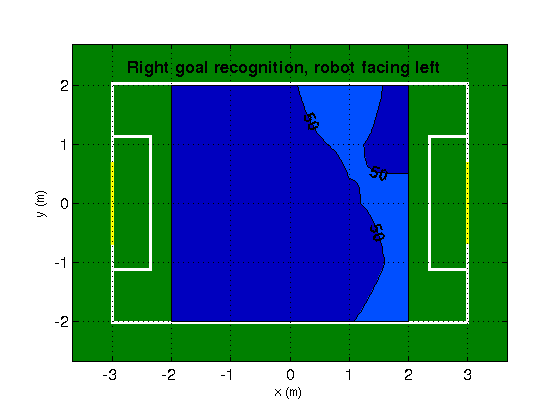
\includegraphics[width=1\textwidth]{figures/RLhard}
\end{minipage}
\begin{minipage}[b]{0.5\textwidth}
\centering
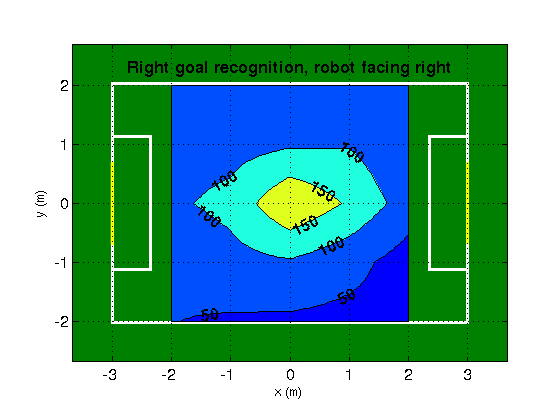
\includegraphics[width=1\textwidth]{figures/RRhard}
\end{minipage}
\begin{minipage}[b]{0.5\textwidth}
\centering
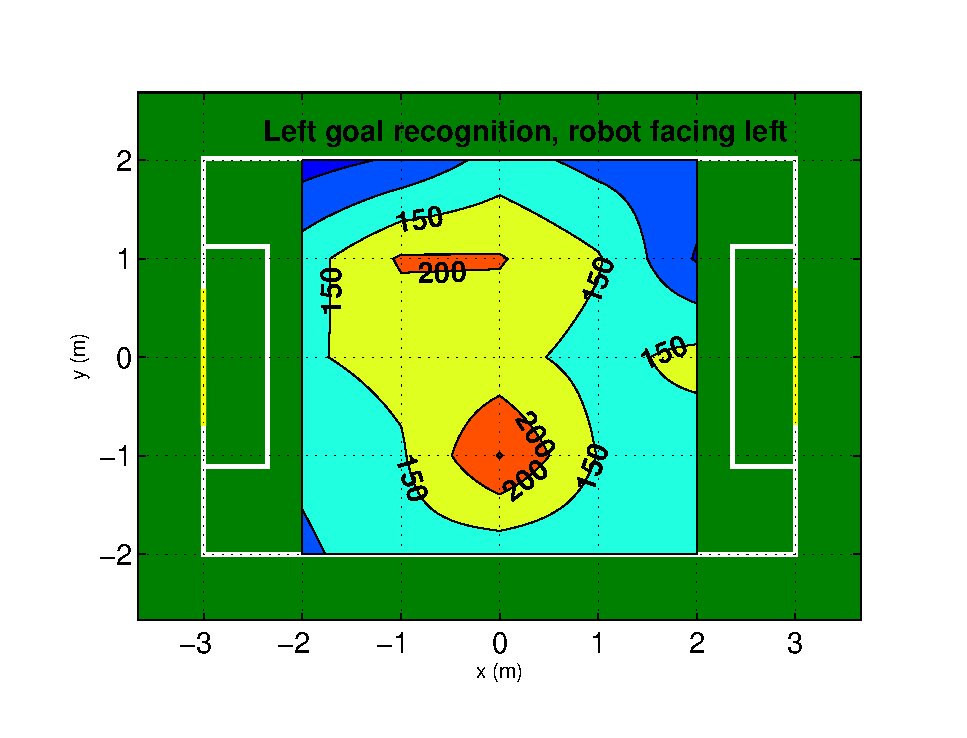
\includegraphics[width=1\textwidth]{figures/LLhard}
\end{minipage}
\begin{minipage}[b]{0.5\textwidth}
\centering
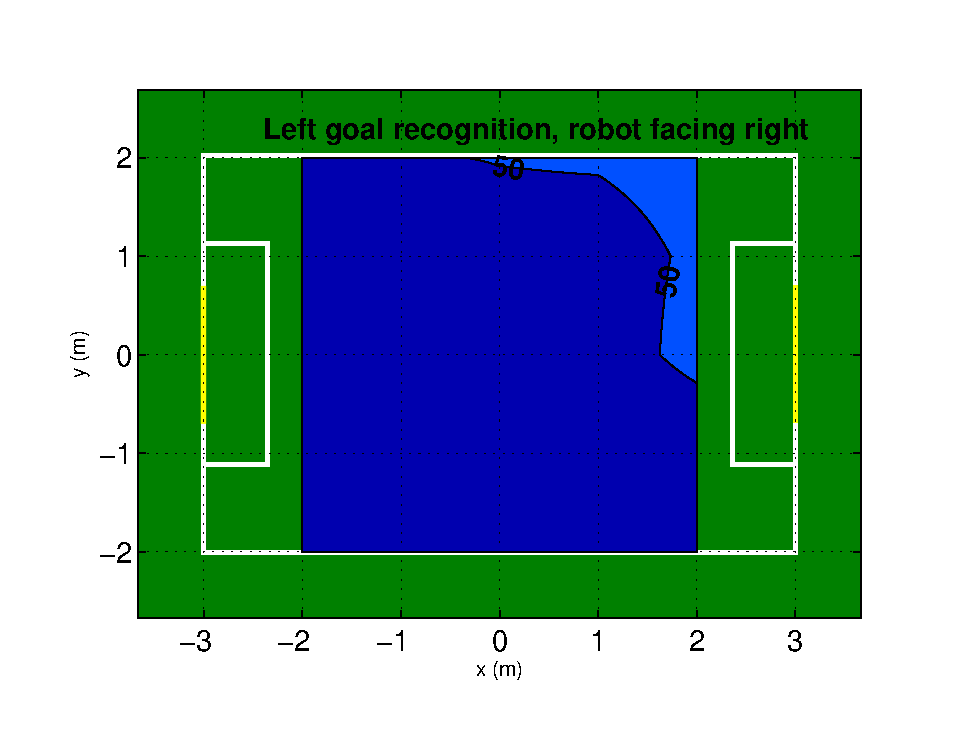
\includegraphics[width=1\textwidth]{figures/LRhard}
\end{minipage}
\caption{Recognition scores of a single goal image from different areas of the field, with the overhead field lighting turned off, and the goals themselves removed. Clockwise from top left: Recognition of right-hand goal when facing left, recognition of right-hand goal when facing right, recognition of left-hand goal when facing right, recognition of left-hand goal when facing left.} \label{fig:heatmaphard}
\end{figure}

\begin{figure} [h]
\begin{minipage}[b]{0.5\textwidth}
\centering
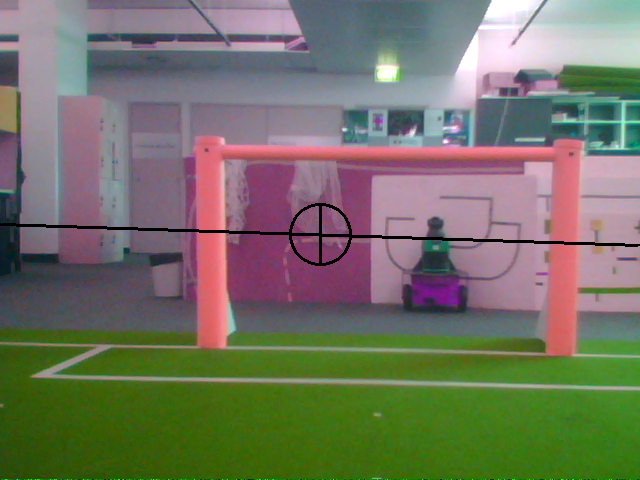
\includegraphics[width=1\textwidth]{figures/img28.png}
\end{minipage}
\begin{minipage}[b]{0.5\textwidth}
\centering
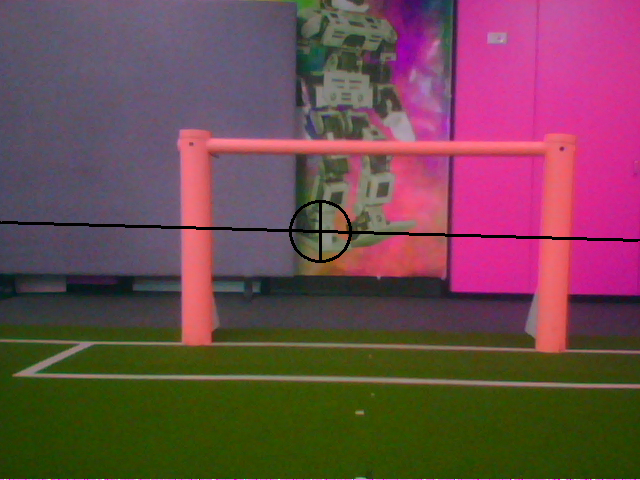
\includegraphics[width=1\textwidth]{figures/img27.png}
\end{minipage}
\begin{minipage}[b]{0.5\textwidth}
\centering
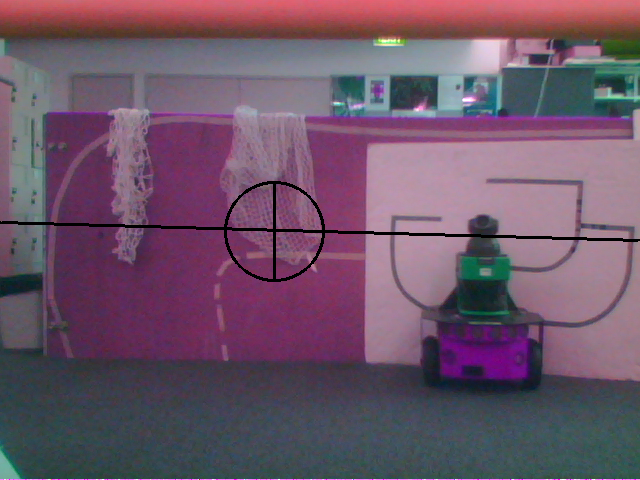
\includegraphics[width=1\textwidth]{figures/img23.png}
\end{minipage}
\begin{minipage}[b]{0.5\textwidth}
\centering
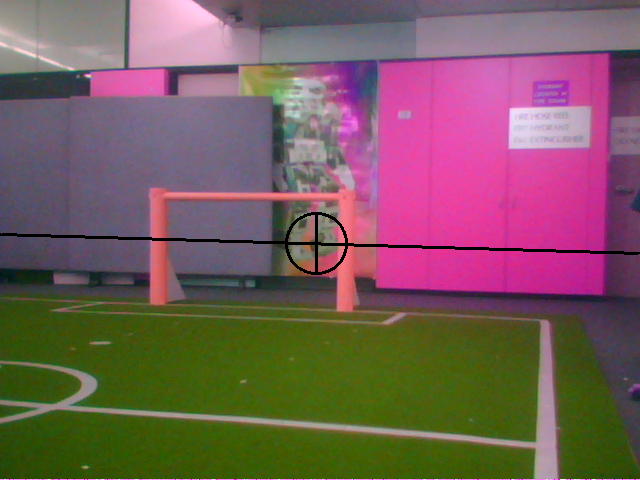
\includegraphics[width=1\textwidth]{figures/img33.png}
\end{minipage}
\begin{minipage}[b]{0.5\textwidth}
\centering
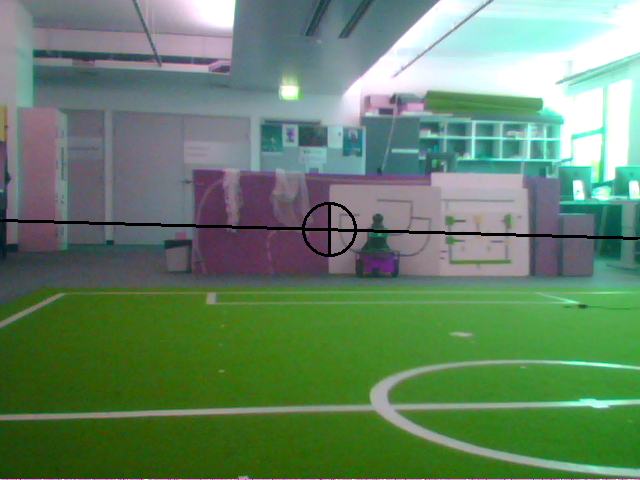
\includegraphics[width=1\textwidth]{figures/img54.png}
\end{minipage}
\begin{minipage}[b]{0.5\textwidth}
\centering
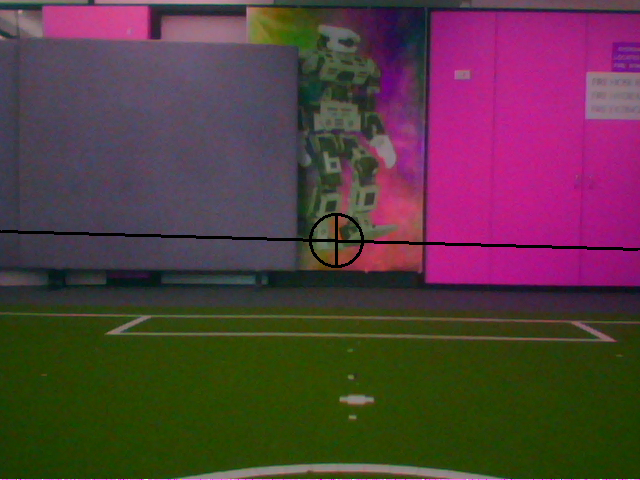
\includegraphics[width=1\textwidth]{figures/img85.png}
\end{minipage}
\begin{minipage}[b]{0.5\textwidth}
\centering
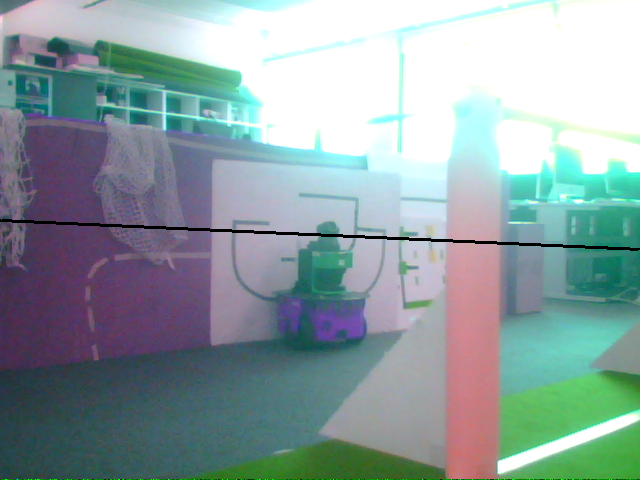
\includegraphics[width=1\textwidth]{figures/img21.png}
\end{minipage}
\begin{minipage}[b]{0.5\textwidth}
\centering
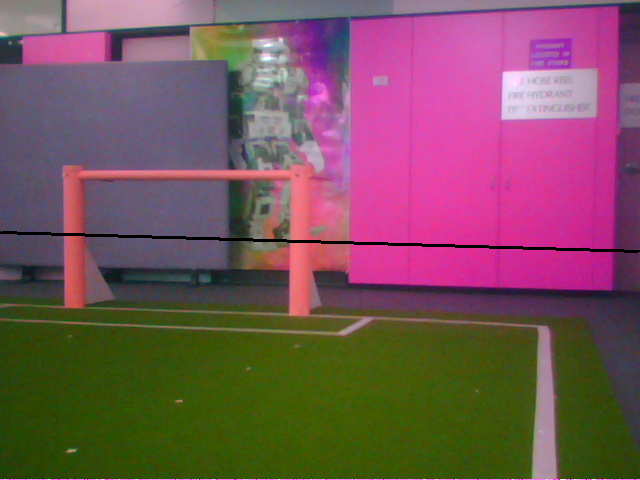
\includegraphics[width=1\textwidth]{figures/img38.png}
\end{minipage}
\caption{Top row: Stored images of the left-hand and right-hand goal areas respectively. Row 2: Examples of correctly matched field views. Markers indicate the scale and position of the match. Row 3: Examples of correctly matched views with goals removed and overhead lights turned off. Bottom row: Some field views that could not be confidently matched to the stored images, possibly due to overexposure and occlusion of key features respectively.} \label{fig:examples}
\end{figure}



\section{Evaluation and Conclusion} \label{sec:conclusions}
This paper has presented an optimised method for extracting local features from 1D images of a mobile robot's horizon. The extracted 1D SURF features are robust to lighting changes, scale changes, and small changes in viewing angle or to the scene itself, making them suitable for robot navigation in indoor environments. Using 1D SURF features and a NN with RANSAC matching technique, we demonstrate that (in a relatively distinctive environment with few scene changes) it is possible to resolve the RoboCup SPL field end ambiguity in real time using just two stored images. 

In actual RoboCup matches, it is likely that the background environment will be more challenging than our laboratory tests due to the coming and going of spectators during the match. As such, we anticipate that in practise it will be necessary to store more than two images, and to update them during the match as the natural landmarks around the field change. In future work we will investigate methods to simultaneously localise and map changing natural landmarks around the field, rather than relying on a fixed set of stored images.

\section{ACKNOWLEDGEMENTS}
The authors gratefully acknowledge the support of the School of Computer Science and Engineering, past and present members of the rUNSWift team, and associated staff and students in the school's robotic laboratory.

\bibliographystyle{plain}
\bibliography{hengst}

\end{document}
